%%%%%%%%InterconnectRT Document%%%%%%%%%%%%%
\documentclass{article}
\usepackage{here}
\usepackage{verbatim}
\usepackage{graphicx}
\oddsidemargin 0.25in \evensidemargin 0.25in
\topmargin 0.0in
\textwidth 6.5in \textheight 8.5in
\headheight 0.18in \footskip 0.16in
\leftmargin -0.5in \rightmargin -0.5in

%
% KEYWORD
%
\newcommand{\keywordtable}[1]{
        \sloppy
        \hyphenation{ca-pac-i-t-an-ce}
        \begin{center}
    \sf
        \begin{tabular}[t]
        {|p{0.58in}|p{3.07in}|p{0.55in}|p{0.60in}|}
        \hline
        \multicolumn{1}{|c}{\bf Name} &
        \multicolumn{1}{|c}{\parbox{2.77in}{\bf Description}}  &
        \multicolumn{1}{|c}{\bf Units} &
        \multicolumn{1}{|c|}{\bf Default} \X
        #1
        \end{tabular}
        \end{center}
    }

\newcommand{\keywordtwotable}[2]{
        \sloppy
        \hyphenation{ca-pac-i-t-an-ce}
        \begin{center}
    \sf
        \begin{tabular}[t]
        {|p{0.58in}|p{2.38in}|p{0.55in}|p{0.60in}|p{0.53in}|}
        \hline
        \multicolumn{1}{|c}{\bf Name} &
        \multicolumn{1}{|c}{\parbox{2.20in}{\bf Description}}  &
        \multicolumn{1}{|c}{\bf Units} &
        \multicolumn{1}{|c}{\bf Default} &
        \multicolumn{1}{|c|}{\bf #1} \X
        #2
        \end{tabular}
        \end{center}
    }

\newcommand{\kw}[2]{
     \samepage{
     \noindent {\sl #1} \vspace{-0.5in} \\
     \keywordtable{#2} }}

\newcommand{\kwtwo}[3]{
     \samepage{
     \noindent {\sl #1} \vspace{-0.4in} \\
     \keywordtwotable{#2}{#3} }}

\newcommand{\keyword}[1]{\kw{Keywords:}{#1}}
\newcommand{\keywordtwo}[2]{\kwtwo{Keywords:}{#1}{#2}}
\newcommand{\modelkeyword}[1]{\kw{Model Keywords}{#1}}
\newcommand{\modelkeywordtwo}[2]{\kwtwo{Model Keywords}{#1}{#2}}

\newcommand{\myline}{\\[-0.1in]
\noindent \rule{\textwidth}{0.01in} \newline}

\newcommand{\myThickLine}{\\[-0.1in]
\noindent \rule{\textwidth}{0.02in} \newline}


% FORM
\newcommand{\form}[1]{\samepage{\noindent
 {\sl Form} \myline
% \hspace*{\fill} % For some reason \fill = 0 when \pspiceform{} is used?
\offset
\it  \offsetparbox{#1}}
\\[0.1in]}

% ELEMENT FORM
\newcommand{\elementform}[1]{\samepage{\noindent
 {\sl Element Form} \myline
% \hspace*{\fill} % For some reason \fill = 0 when \pspiceform{} is used?
\offset
\it  \offsetparbox{#1}}
\\[0.1in]}

% MODEL FORM
\newcommand{\modelform}[1]{\samepage{\noindent
 {\sl Model Form} \myline
% \hspace*{\fill} % For some reason \fill = 0 when \pspiceform{} is used?
\offset
\it  \offsetparbox{#1}}
\\[0.1in]}

% LIMITS
\newcommand{\mylimits}[1]{\samepage{\noindent
 {\sl Limits} \myline
 \hspace*{\fill} \it  \offsetparbox{#1}}
 \vshift}

% EXAMPLE
\newcommand{\example}[1]{\samepage{\noindent
{\sl Example} \myline
\offset \tt  \offsetparbox{#1}}
 \vshift}

% PSPICE88 EXAMPLE
\newcommand{\pspiceexample}[1]{\samepage{\noindent
{\sl \pspice\ Example} \myline
\offset \tt  \offsetparbox{#1}}
 \vshift}

% MODEL TYPES
\newcommand{\modeltype}[1]{\samepage{\noindent
{\sl Model Type} \myline
 \hspace*{\fill} \tt \offsetparbox{#1}}
 \\[0.1in]}

% MODEL TYPES
\newcommand{\modeltypes}[1]{\samepage{\noindent
{\sl Model Types:} \myline
 \hspace*{\fill} \tt \offsetparbox{\tt #1}}
 \vshift}

% OFFSET ENUMERATE
\newcommand{\offsetenumerate}[1]{
     \offset \hspace*{-0.1in} {\begin{enumerate} #1 \end{enumerate}}}

% NOTE
\newcommand{\note}[1]{
\vshift\samepage{\noindent {\sl Note}\myline\vspace{-0.24in}}
 \offsetenumerate{#1} }

% SPECIAL NOTE
\newcommand{\specialnote}[2]{
\vshift\samepage{\noindent {\sl #1}\myline\vspace{-0.24in}}\\#2}

\newcommand{\dc}{\mbox{\tt DC}}
\newcommand{\ac}{\mbox{\tt AC}}
\newcommand{\SPICE}{\mbox{\tt SPICE}}
\newcommand{\m}[1]{{\bf #1}}                           % matrix command  \m{}

% ////// Changing nodes to terminals///////
% print terminals in \tt and enclose in a circle use outside
\newcommand{\terminal}[1]{\: \mbox{\tt #1} \!\!\!\! \bigcirc }
%
% set up environment for example
%
\newcounter{excount}
\newcounter{dummy}
\newenvironment{eg}{\vspace{0.1in}\noindent\rule{\textwidth}{.5mm}
   \begin{list}
   {{\addtocounter{excount}{1}
   \em Example\/ \arabic{chapter}.\arabic{excount}\/}:}
   {\usecounter{dummy}
   \setlength{\rightmargin}{\leftmargin}}
   }{\end{list} \rule{\textwidth}{.5mm}\vspace{0.1in}}
%
% set up environment for block
% currently this draws a horizontal line at the start of block and another
% at the end of block.
%
\newenvironment{block}{\vspace{0.1in}\noindent\rule{\textwidth}{.5mm}
   }{\rule{\textwidth}{.5mm}\vspace{0.1in}}
%


%
% set up wide descriptive list
%
\newenvironment{widelist}
    {\begin{list}{}{\setlength{\rightmargin}{0in} \setlength{\itemsep}{0.1in}
    \setlength{\labelwidth}{0.95in} \setlength{\labelsep}{0.1in}
\setlength{\listparindent}{0in} \setlength{\parsep}{0in}
    \setlength{\leftmargin}{1.0in}}
    }{\end{list}}

\newcommand{\STAR}{\hspace*{\fill} * \hspace*{\fill}}

\newcommand{\sym}[1]{\hspace*{\fill} ($#1$)}

\newcommand{\optionitem}[2]{
\item[{\tt #1}{#2}]\label{.OPTION#1}\index{.OPTIONS, #1}\index{#1}}

\newcommand{\error}[1]{\vspace{0.1in}\noindent{\tt #1}\\}


\begin{document}
\noindent{\LARGE \textbf{Resistive Thermal Interconnect}
\hspace{\fill}\textbf{interconnectrt}}
\myThickLine
\normalsize
\newline
% the interconnect figure
\begin{figure}[h]
\centerline{
\includegraphics[scale=1.5]{interconnectrt.eps}} \caption{interconnectrt --- Resistive
electro-thermal interconnect element.}
\end{figure}
\newline
Author: Kai Li
\newline
\myThickLine
\newline
Description:\newline
This element implements an interconnect line as an electro-thermal resistor. effects.
\newline
\myThickLine
\newline
\textit{Form:}
%\newline
$\tt interconnectrt$:$\langle \tt{instance\ name}\rangle$ $n_1\ n_2\ n_3\
n_4\ $ $\langle \tt{parameter\ list}\rangle$
\newline
\bigskip
\begin{tabular}{l}
instance name is the model name,\\
$n_1$, $n_2$, $n_3$ and $n_4$ are the element terminals, \\
$n_1$ and $n_2$ are element electrical terminals, \\
$n_3$ and $n_4$ are element thermal terminals, \\
$n_2$ is the element local reference node,\\
$n_4$ is the element thermal reference node. \\
\end{tabular}
% Parameter list
\newline
\myThickLine
\textit{Parameters:}
\begin{table}[H]
\begin{tabular}{|c|c|c|c|}
\hline
Parameter&Type&Default value&Required?\\
\hline
l: Length of interconnect line (m) & DOUBLE &  n/a & yes \\
\hline
w: Width of interconnect line (m) & DOUBLE & 1 $\mu m$ & no \\
\hline
tm: Thickness of interconnect line (m) & DOUBLE & 0.3 $\mu m$  & no \\
\hline
rho: Resistivity of metal  ($\Omega-m$)& DOUBLE & n/a & no \\
\hline
metal: Metal (Silver, Copper, Gold, Aluminum) & STRING & copper & no \\
\hline
t: System temperature ($^0C$) & DOUBLE & 20 & no \\
\hline
tnom: Initial system temperature ($^0C$) & DOUBLE & 20 & no \\
\hline
tc: Temperature coefficient (1/$^0C$) & DOUBLE & 0 & no \\
\hline
pdr:  Thermal element flag & BOOLEAN & false & no \\
%\\hline
%idf: Ideality factor of resistance & DOUBLE & 0.8 & no\\
\par
\hline
\end{tabular}
\end{table}
% example in FREEDA
\noindent\myThickLine
\newline
\textit{Example:}
\newline
\texttt{interconnectrt:\ irt1\ 2\ 0\ 3\ "tref" \ l = 20u \ metal = "copper"}
\newline
\myThickLine
\textit{Details:}\\
The resistive thermal interconnect is modeled as resistive only, the metal line is made by a kind of metal, which includes silver, copper, gold, and aluminum that are predefined in the model. \\

\noindent This is an electro-thermal element  is modeled differently depending on the setting of the Parameter \texttt{pdr}.\\[0.2in]
\texttt{pdr} = false/true.\\[0.1in]
 When  \texttt{pdr} is false (the default) the interconnect line is calculated as a resistor by giving length and resistivity or metal selection.\\
 When  \texttt{pdr} is true, the interconnect line is modeled as electro-thermal resistor by giving length, resistivity or metal selection, and system temperature. Resistance calculation is based on the electrical parameters and system temperature. The power dissipation and heat flux are modeled with thermal terminals.\\[0.1in]
 \newline
 Resistance of the interconnect line:\\
 $$R\,=\, \frac{\rho \cdot l}{A}$$
\newline
Electro-thermal resistance of the interconnect with temperature coefficient:
$$R \,=\, \frac{\rho \cdot l}{A}  \cdot \left[  1\, + \, \beta \cdot  (\, t\, - t_0\,) \right] $$
\begin{verbatim}
interconnectrt: irt1 2 0 3 "tref" l = 20u  metal = "copper"
\end{verbatim}
Here terminals `0' and `tref' are the local reference terminals of the element. Terminal `0' is the global ground.  Terminal 'tref' is a thermal local reference terminal of the element. An example netlist is:
\begin{verbatim}
.ref "tref"
.ref 0

vsource 1 0 vac = 1 f = 5GHz
res:r1 1 2 r=50
interconnectrt:irt1 2 0 1000 "tref" l = 1m metal = "copper" pdr=1
\end{verbatim}
~
\myThickLine
\textit{References:}\\
\begin{enumerate}
\item Houssam S.Kanj. fREEDA element ResistorT, $"elements\backslash r\backslash ResistorT$".
\item Tony Mulder, Travis Lentz. fREEDA element CmosInvT, "$elements\backslash c\backslash CmosInvT$"
\end{enumerate}
~
\myThickLine
Example of Transient Analysis (.TRAN2) Fixed times steps, time-stepping nonlinear analysis.\\
netlist file: interconnectrt.net:
\verbatiminput{../test/interconnectrt.net}
The output log file is
\verbatiminput{../test/interconnectrt.out}
\begin{figure}[h]
\centerline{\includegraphics[width=4in]{trans_res.eps}}\caption{Transient Analysis - Resistance variation of thermal interconnect}
\centerline{\includegraphics[width=4in]{trans_temp.eps}}\caption{Transient Analysis - Temperature variation of interconnect line}
\end{figure}
\clearpage
~
\myThickLine
\textit{Version:}\\
2008.04.21 (2008 April 21) \\
% Credits
\myThickLine
\medskip
\textit{Credits:}\\
\begin{tabular}{l  l  l  l}
Name & Affiliation & Date & Links \\
Kai Li & NC State University & April 2008 & 
\includegraphics[width=1in]{logo.eps}  \\
kli@ieee.org & & & www.ncsu.edu    \\
\end{tabular}
\end{document}
